% Author: Rasmus Pank Roulund
\documentclass[tikz]{standalone}

%adapted from http://tex.stackexchange.com/questions/167483/spanning-a-cell-across-several-rows-in-tikz-matrix

\usetikzlibrary{calc,trees,positioning,arrows,chains,shapes.geometric,%
    decorations.pathreplacing,decorations.pathmorphing,shapes,%
    matrix,shapes.symbols,fit}

\pgfdeclarelayer{back}
\pgfsetlayers{back,main}

\tikzstyle{block} = [draw, fill=blue!20, rectangle, 
    minimum height=3em, minimum width=4em]

\tikzstyle{wblock} = [draw, rectangle, 
    minimum height=3em, minimum width=4em]


\begin{document}
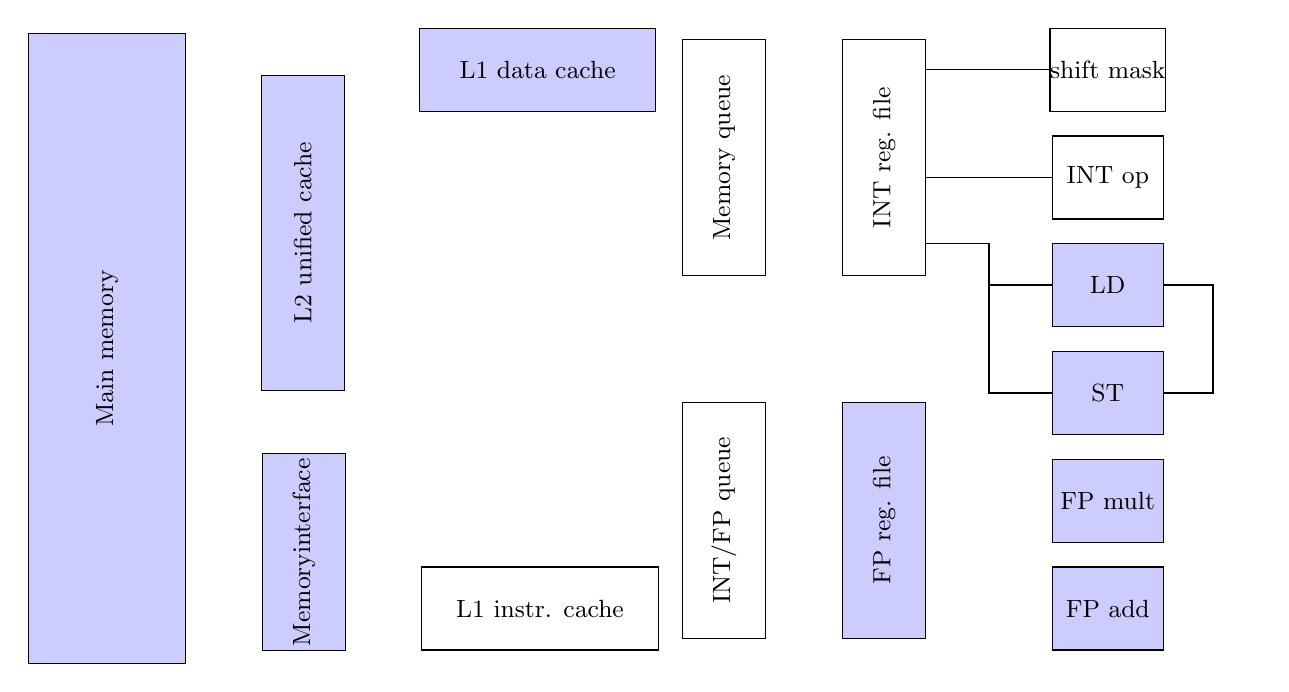
\begin{tikzpicture}[auto, node distance=2.5cm,>=latex',font=\small,
    every node/.style={inner sep=0pt,rectangle, minimum height=2.5em, text centered}]
    \matrix (m) [ampersand replacement=\&,column sep=6mm, row sep=3mm]
    {
      \node (leftof_sm) [coordinate] {}; \& \node (sm) [wblock] {shift\newline{} mask}; \& 
 \\
      \node (leftof_intop) [coordinate] {}; \& \node (intop) [wblock] {INT\newline{} op}; \& 
 \\
      \node (leftof_ld) [coordinate] {}; \& \node (ld) [block] {LD}; \& \node (rightof_ld) [coordinate] {}; \&
 \\
      \node (leftof_st) [coordinate] {}; \& \node (st) [block] {ST}; \& \node (rightof_st) [coordinate] {}; \&
 \\
      \node (leftof_fpmult) [coordinate] {}; \& \node (fpmult) [block] {FP\newline{} mult}; \&
 \\
      \node (leftof_fpadd) [coordinate] {}; \& \node (fpadd) [block] {FP\newline{} add}; \&
 \\
    };

\node (intregfile) [wblock,rotate=90,minimum width=3cm] at($(leftof_intop.west) + (-1.5cm,.25cm)$) {INT reg. file};
\node (fpregfile) [block,rotate=90,minimum width=3cm] at($(leftof_fpmult.west) - (1.5cm,.25cm)$) {FP reg. file};

\node (fpregfile_hi_right) [coordinate] at($(fpregfile.south east)!.33!(fpregfile.south west)$) {};
\node (fpregfile_lo_right) [coordinate] at($(fpregfile.south east)!.66!(fpregfile.south west)$) {};



%\path let \p1 = (A) in node  at (\x1,3) {B};
%\draw (A |- 52,3) node {B};
%\path ($(sm.east)$) edge[-] () ;%

%manual, p.152
\path 
let
\p1
 = ($(sm.west)$),
\p2
 = ($(intregfile.south)$),
\p3
 = ($(intop.west)$),
\p4
 = ($(ld.north)$),
\p5
 = ($(ld.west)$),
\p6
 = ($(st.west)$),
\n1 = {\x2 + abs(\x5-\x2)/2}
in
coordinate
 (intregfile_hi_right) at (\x2,\y1)
coordinate
 (intregfile_mi_right) at (\x2,\y3)
coordinate
 (intregfile_lo_right) at (\x2,\y4)
coordinate
 (junctn_ld_north) at (\n1,\y4)
coordinate
 (junctn_ld_west) at (\n1,\y5)
coordinate
 (junctn_st_west) at (\n1,\y6);

\draw[-] ($(sm.west)$) -- (intregfile_hi_right);
\draw[-] ($(intop.west)$) -- (intregfile_mi_right);
\draw[-] (intregfile_lo_right) -| (junctn_ld_north) -- (junctn_ld_west);
\draw[thick,-] ($(ld.west)$) |- (junctn_ld_west) -- (junctn_st_west) |- ($(st.west)$);



\draw[thick,-] ($(ld.east)$) |- (rightof_ld) -- (rightof_st) |- ($(st.east)$);


\node (memqueue) [wblock,rotate=90,minimum width=3cm] at($(intregfile.north) - (1.5cm,0cm)$) {Memory queue};
\node (intfpqueue) [wblock,rotate=90,minimum width=3cm] at($(fpregfile.north) - (1.5cm,0cm)$) {INT/FP queue};


\node (intregfile_hi_left) [coordinate] at($(intregfile.north east)!.33!(intregfile.north west)$) {};
\node (intregfile_lo_left) [coordinate] at($(intregfile.north east)!.66!(intregfile.north west)$) {};
\node (fpregfile_lo_left) [coordinate] at($(fpregfile.north east)!.66!(fpregfile.north west)$) {};


\node (l1d) [block,minimum width=3cm] at($(sm.west) + (-6.5cm,0cm)$) {L1 data cache};
\node (l1i) [wblock,minimum width=3cm] at($(fpadd.west) + (-6.5cm,0cm)$) {L1 instr. cache};


\node (ram) [block,rotate=90,minimum width=8cm, minimum height=2cm] at($(fpadd.west) + (-12.cm,3.3cm)$) {Main memory};

\node (vRAM1) [coordinate] at($(ram.south east)!.4!(ram.south)$) {};
\node (vRAM2) [coordinate] at($(ram.south west)!.4!(ram.south)$) {};

\node (l2cache) [block,rotate=90,minimum width=4cm] at($(l1d.west)!.5!(vRAM1) + (0,-1.5cm)$) {L2 unified cache};
\node (memif) [block,rotate=90,minimum width=2.5cm] at($(l1i.north west)!.5!(vRAM2)$) {Memory\newline{}interface};

% \coordinate (aux1) at (D.west |- A.north);
% \coordinate (aux2) at ($(C.south west) - (3mm,0mm)$);
% \node[block, fit=(aux1)(aux2), inner sep=-.6pt] (X) {}; 
% \node[text width=3cm, text centered, anchor=center, rotate=90] at (X.center) {Main memory};


  \end{tikzpicture}
\end{document}
%%% Local Variables: 
%%% mode: latex
%%% TeX-master: t
%%% End: 
